% !Mode:: "TeX:UTF-8"
% !TEX program  = xelatex
%\documentclass{cumcmthesis}



% ***************************************************************************************

                % *********    ******     ********
                % **         **          **      
                % **         **         **
                % *********    ******  **
                % **               **   **
                % **               **    **
                % **         ******       ********

% This Latex example is refactored from CUMCM by FSC(https://github.com/fscdc), Feel Free to use! 
% This example is used for 生态文明导论论文 at present and can be extended into many different paper example in Chinese! Make it into TODO for now

% ***************************************************************************************




\documentclass[withoutpreface,bwprint]{cumcmthesis}
\usepackage[framemethod=TikZ]{mdframed}
\usepackage{url}   
\usepackage{subcaption} 
\title{\zihao{4}本科生2023—2024学年第二学期\\生态文明建设课程期末考试试卷(论文)}
%'''
\usepackage{amsmath}   % Package for math files
\usepackage{txfonts}
\usepackage{graphicx}  % Place figures
\usepackage{caption}   % Place captions in tables and figures
\usepackage{subcaption}% 
\usepackage{placeins}  % \FloatBarrier so figures can't float beyond some point in text
% \usepackage{fullpage}  % Uses more of the page
\usepackage{float}     % Able to make figures and tables float
%表格自动生成
\usepackage{subfloat}
\usepackage{subcaption} 
\usepackage{subfiles}  
\usepackage{hyperref} 
 % Ability to click on references like equations, figures, sections etc. \ref{eq:my_eq} clickable
\usepackage{placeins}  
% \FloatBarrier so figures can't float beyond some point in text
\usepackage[T1]{fontenc} 
%英文字体定义
\usepackage{setspace}

\setstretch{1.0} % 将行间距设置为单倍行距
\usepackage{titlesec}
\titleformat{\section}[block]{\zihao{-4}\bfseries\setstretch{1.5}}{\thesection}{1em}{}
\titleformat{\subsection}[block]{\zihao{-4}\bfseries\setstretch{1.5}}{\thesubsection}{1em}{}
\titleformat{\subsubsection}[block]{\zihao{-4}\bfseries\setstretch{1.5}}{\thesubsubsection}{1em}{}
\titleformat{\paragraph}[block]{\zihao{-4}\bfseries\setstretch{1.5}}{\theparagraph}{1em}{}

%''' 

\usepackage{titlesec}
% 重定义章节段的行间距和字体
\titleformat{\section}[block]{\zihao{-4}\bfseries\setstretch{1.5}}{\thesection}{1em}{}
\titleformat{\subsection}[block]{\zihao{-4}\bfseries\setstretch{1.5}}{\thesubsection}{1em}{}
\titleformat{\subsubsection}[block]{\zihao{-4}\bfseries\setstretch{1.5}}{\thesubsubsection}{1em}{}
\titleformat{\paragraph}[block]{\zihao{-4}\bfseries\setstretch{1.5}}{\theparagraph}{1em}{}

%'''
% \renewcommand {\thetable} {\thechapter{}.\arabic{table}}
% %表格根据章节自动命名
% \renewcommand {\thefigure} {\thechapter{}.\arabic{figure}}
% %图片根据章节自动命名

\renewcommand {\thetable} {\arabic{table}}
\renewcommand {\thefigure} {\arabic{figure}}

% \numberwithin{figure}{section}
% \numberwithin{table}{section}
\numberwithin{equation}{section}
%以上三个皆控制重命名
\newcommand{\figref}[1]{\figurename~\ref{#1}} 
% 定义正常字体就是五号字体
\renewcommand{\normalsize}{\zihao{5}}
%Nice reference to figures

\hypersetup{
    colorlinks,
    citecolor=blue,
    filecolor=blue,
    linkcolor=blue,
    urlcolor=blue
}
%'''


\begin{document}



\maketitle


% 这个是用于复现出生态文明导论的封面,如果您用于其他课程,可自行进行调整
\begin{center}
    {\zihao{-4}
    \begin{tabular}{lp{3.5cm}lp{3.5cm}lp{3.5cm}lp{3cm}lp{2cm}lp{3.5cm}lp{2cm}l}
        \textbf{专业:} & 计算机科学与技术  & \textbf{年级:}   & 大六           &      &  \\
        \textbf{学号:} & 1234567 & \textbf{姓名:} & 无敌龙帝  & \textbf{成绩:} & 棒极了 \\
    \end{tabular}
    }
    \vspace{0.8cm}
\end{center}

\newpage

\begin{center}
    \begin{spacing}{1.5} % 设置行间距为1.5倍
        {\hei \zihao{3}\textbf{这是一个标题}}
    \end{spacing}
\end{center}

% 这里需要注意下这个标题需要您最后自己手动换成黑体,不知道为什么我的黑体命令不生效,目前还没debug出来


\begin{abstract}
        我想在那里待上一整天这是一个美好的地方今天天气真好我想去公园散步在那里可以看到很多树木和花朵我喜欢听到鸟儿在树上唱歌它们的声音很美妙我也喜欢看到小溪流过水的颜色很清澈我想在那里待上一整天这是一个美好的地方今天天气真好我想去公园散步在那里可以看到很多树木和花朵我喜欢听到鸟儿在树上唱歌它们的声音很美妙我也喜欢看到小溪流过水的颜色很清澈我想在那里待上一整天这是一个美好的地方今天天气真好我想去公园散步在那里可以看到很多树木和花朵我喜欢听到鸟儿在树上唱歌它们的声音很美妙我也喜欢看到小溪流过水的颜色很清澈我想在那里待上一整天,这是一段摘要。
	\keywords{\quad Latex \quad 生态文明 \quad  }
\end{abstract}

% 您也可以使用英文摘要,请您根据需求自行调整。
% \renewcommand{\abstractname}{Abstract}
% \renewcommand{\keywords}{\textbf{Keywords:}}
% \newpage

% \begin{abstract}
% \begin{spacing}{1.6}

% \end{spacing}
% \noindent\keywords{Frequency Selective Surface\quad Polarization Insensitivity\quad Three-layer Composite Structure}
% \end{abstract}


% 目录根据您的需求自行调整
% \newpage
% \tableofcontents
% \newpage

% 这里section、subsection、subsubsection可以直接命名即可,标号会自动添加,但是paragraph需要您像下文中写一下即可。

\section{第一部分}

\subsection{第一小节}

\subsubsection{第一小小节}

\paragraph{(1) \quad 第一段}



正文、加粗、斜体示例:新中国是红色的,\textbf{新中国是红色的},\textit{新中国是红色的} 

引用示例:(三种不同的引用风格,您自行选取)
\cite{theodoris2023transfer} \upcite{theodoris2023transfer} \supercite{theodoris2023transfer}


换行示例:\\哈哈哈哈哈哈

这是一个分点示例:

\begin{itemize}
    \item 
    \item 
\end{itemize}


\newpage

今天天气真好我想去公园散步在那里可以看到很多树木和花朵我喜欢听到鸟儿在树上唱歌它们的声音很美妙我也喜欢看到小溪流过水的颜色很清澈我想在那里待上一整天这是一个美好的地方今天天气真好我想去公园散步在那里可以看到很多树木和花朵我喜欢听到鸟儿在树上唱歌它们的声音很美妙我也喜欢看到小溪流过水的颜色很清澈我想在那里待上一整天这是一个美好的地方今天天气真好我想去公园散步在那里可以看到很多树木和花朵我喜欢听到鸟儿在树上唱歌它们的声音很美妙我也喜欢看到小溪流过水的颜色很清澈我想在那里待上一整天这是一个美好的地方今天天气真好我想去公园散步在那里可以看到很多树木和花朵我喜欢听到鸟儿在树上唱歌它们的声音很美妙我也喜欢看到小溪流过水的颜色很清澈我想在那里待上一整天这是一个美好的地方今天天气真好我想去公园散步在那里可以看到很多树木和花朵我喜欢听到鸟儿在树上唱歌它们的声音很美妙我也喜欢看到小溪流过水的颜色很清澈我想在那里待上一整天这是一个美好的地方今天天气真好我想去公园散步在那里可以看到很多树木和花朵我喜欢听到鸟儿在树上唱歌它们的声音很美妙我也喜欢看到小溪流过水的颜色很清澈我想在那里待上一整天这是一个美好的地方今天天气真好我想去公园散步在那里可以看到很多树木和花朵我喜欢听到鸟儿在树上唱歌它们的声音很美妙我也喜欢看到小溪流过水的颜色很清澈我想在那里待上一整天这是一个美好的地方今天天气真好我想去公园散步在那里可以看到很多树木和花朵我喜欢听到鸟儿在树上唱歌它们的声音很美妙我也喜欢看到小溪流过水的颜色很清澈我想在那里待上一整天这是一个美好的地方今天天气真好我想去公园散步在那里可以看到很多树木和花朵我喜欢听到鸟儿在树上唱歌它们的声音很美妙我也喜欢看到小溪流过水的颜色很清澈我想在那里待上一整天这是一个美好的地方今天天气真好我想去公园散步在那里可以看到很多树木和花朵我喜欢听到鸟儿在树上唱歌它们的声音很美妙我也喜欢看到小溪流过水的颜色很清澈我想在那里待上一整天这是一个美好的地方今天天气真好我想去公园散步在那里可以看到很多树木和花朵我喜欢听到鸟儿在树上唱歌它们的声音很美妙我也喜欢看到小溪流过水的颜色很清澈我想在那里待上一整天这是一个美好的地方今天天气真好我想去公园散步在那里可以看到很多树木和花朵我喜欢听到鸟儿在树上唱歌它们的声音很美妙我也喜欢看到小溪流过水的颜色很清澈我想在那里待上一整天这是一个美好的地方今天天气真好我想去公园散步在那里可以看到很多树木和花朵我喜欢听到鸟儿在树上唱歌它们的声音很美妙我也喜欢看到小溪流过水的颜色很清澈我想在那里待上一整天这是一个美好的地方今天天气真好我想去公园散步在那里可以看到很多树木和花朵我喜欢听到鸟儿在树上唱歌它们的声音很美妙我也喜欢看到小溪流过水的颜色很清澈我想在那里待上一整天这是一个美好的地方今天天气真好我想去公园散步在那里可以看到很多树木和花朵我喜欢听到鸟儿在树上唱歌它们的声音很美妙我也喜欢看到小溪流过水的颜色很清澈我想在那里待上一整天这是一个美好的地方今天天气真好我想去公园散步在那里可以看到很多树木和花朵我喜欢听到鸟儿在树上唱歌它们的声音很美妙我也喜欢看到小溪流过水的颜色很清澈我想在那里待上一整天这是一个美好的地方今天天气真好我想去公园散步在那里可以看到很多树木和花朵我喜欢听到鸟儿在树上唱歌它们的声音很美妙我也喜欢看到小溪流过水的颜色很清澈我想在那里待上一整天这是一个美好的地方今天天气真好我想去公园散步在那里可以看到很多树木和花朵我喜欢听到鸟儿在树上唱歌它们的声音很美妙我也喜欢看到小溪流过水的颜色很清澈我想在那里待上一整天这是一个美好的地方今天天气真好我想去公园散步在那里可以看到很多树木和花朵我喜欢听到鸟儿在树上唱歌它们的声音很美妙我也喜欢看到小溪流过水的颜色很清澈我想在那里待上一整天
澈我想在那里待上一整天澈我想在那里待上一整天澈我想在那里待上一整天颜色很清澈我想在那里待上一整天这是一个美好的地方今天天气真好我想去公园好里待上一整天澈我想在那里待上一整天颜色很清澈我想在那里待上一整天这是一个美好的地方今天天气真好我想去公园好里待上一整天澈我想在那里待上一整天颜色很清澈我想在那里待上一整天这是一个美好的地方今天天气真好我想去公园好里待上一整安抚我撒旦哇噶日嘎尔。在树上唱歌它们的声音很美妙我也喜欢看到小溪流过水的颜色很清澈我想在那里待上一整天这是一个美好的地方今天天气真好我想去公园散步在那里可以看到很多树木和花朵我喜欢听到鸟儿在树上唱歌它们的声音很美妙我也喜欢看到小溪流过水的颜色很清澈我想在那里待上一整天这是一个美好的地方今天天气真好我想去公园散步在那里可以看到很多树木和花朵我喜欢听到鸟儿在树上唱歌它们的声音很美妙我也喜欢看到小溪流过水的颜色很清澈我想在那里待上一整天这是一个美好的地方今天天气真好我想去公园散步在那里可以看到很多树木和花朵我喜欢听到鸟儿在树上唱歌它们的声音很美妙我也喜欢看到小溪流过水的颜色很清澈我想在那里待上一整天这是一个美好的地方今天天气真好我想去公园散步在那里可以看到很多树木和花朵我喜欢听到鸟儿在树上唱歌它们的声音很美妙我也喜欢看到小溪流过水的颜色很清澈我想在那里待上一整天这是一个美好的地方今天天气真好我想去公园散步在那里可以看到很多树木和花朵我喜欢听到鸟儿在树上唱歌它们的声音很美妙我也喜欢看到小溪流过水的颜色很清澈我想在那里待上一整天这是一个美好的地方今天天气真好我想去公园散步在那里可以看到很多树木和花朵我喜欢听到鸟儿在树上唱歌它们的声音很美妙我也喜欢看\\


表格示例:

\begin{table}[H]
  \centering 
  \caption{实验工具说明表}
  \begin{tabular}{ccccccccccc}
  \toprule  
  vs code版本&  Perf版本&  g++版本\\
  \midrule
  1.86.2(Windows)/1.82.2(L) & 6.5.8(L)/4.18.0(ARM) & 8.1.0(Windows)/11.4.0(L)/9.3.1(ARM) \\
  \bottomrule
  \end{tabular}
\end{table}


\begin{figure}[!htbp]
    \centering
    \caption{这是一个示例图}
    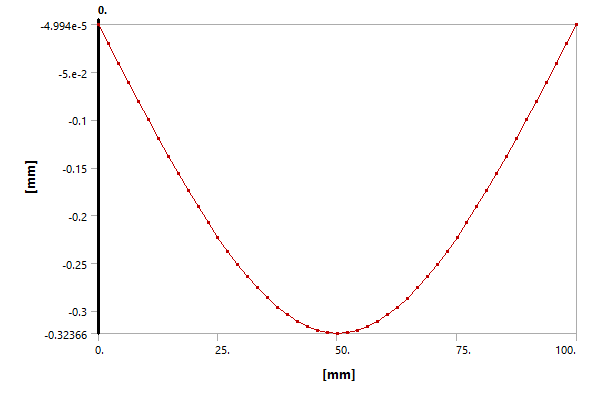
\includegraphics[scale=0.5]{Figure/example.png}
\end{figure}


\begin{figure}[!htbp]
    \centering
    \caption{这也是一个示例图}
    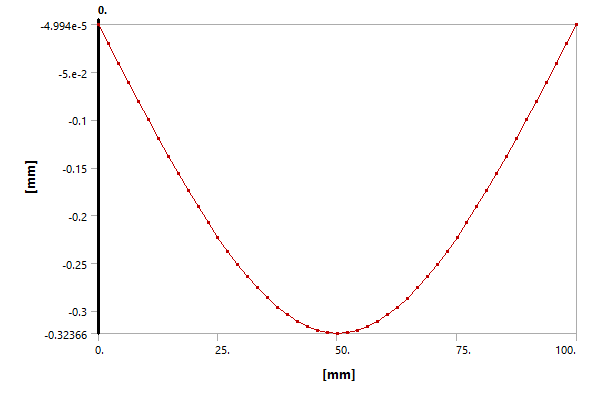
\includegraphics[scale=0.5]{Figure/example.png}
\end{figure}


%参考文献,这里添加引用的方式为,您需要将论文的bibtex添加到cite.bib文件中,然后在下面添加一下,再然后按照您需要的格式自行引用即可,上文中有引用的example。
\newpage
\begin{thebibliography}{cite.bib}
    \bibitem{theodoris2023transfer}
    Theodoris, C.V., Xiao, L., Chopra, A., Chaffin, M.D., Al Sayed, Z.R., Hill, M.C., Mantineo, H., Brydon, E.M., Zeng, Z., Liu, X.S. and Ellinor, P.T., 2023. Transfer learning enables predictions in network biology. Nature, 618(7965), pp.616-624.
    

\end{thebibliography}

%附录
% Appendix
%\appendix
%\pagenumbering{roman}


\end{document} 